Für einen \ct{} muss also die gemeinsame und disjunkte Nachbarschaft bestimmt 
und die disjunkte Nachbarschaft zufällig durchmischt werden.
Die Nachbarschaften eines jeden Knotens sind jeweils in einem Array gespeichert. 
%
%
%
%
%
%
%%%%% CURVEBALL TRADE auf Array
\begin{figure}[H]
\centering
  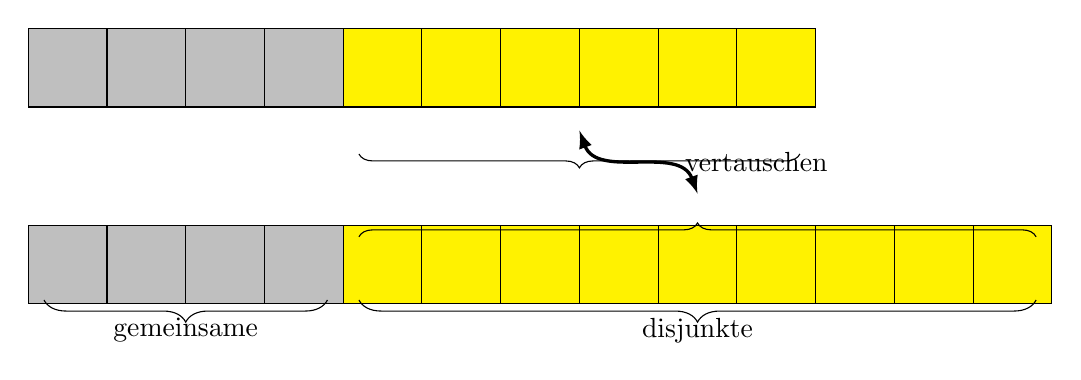
\begin{tikzpicture}[decoration=brace]
      
      
    %% COMMON FÄRBEN  
    \foreach \x in {0,1,2,3}
		{
			\fill [ fill =lightgray, draw =black ]  (\x ,0) rectangle (\x+1 ,1) ;
			\fill [ fill =lightgray, draw =black ]  (\x ,-2.5) rectangle (\x+1 ,-1.5) ;
		};

    %% DISJOINT OBEN FÄRBEN  
    \foreach \x in {4,5,6,7,8,9}
		{
			\fill [ fill =yellow, draw =black ]  (\x ,0) rectangle (\x+1 ,1) ;
		};
		
	%% DISJOINT UNTEN FÄRBEN  
    \foreach \x in {4,5,6,7,8,9,10,11,12}
		{
			\fill [ fill =yellow, draw =black ]  (\x ,-2.5) rectangle (\x+1 ,-1.5) ;
		};
    
%\node[] at (-0.8, 0.5)     (5)     {$N(u):$};
%\node[] at (-0.8, -2)     (5)     {$N(v):$};
    
    \draw[decorate, yshift=+2ex,decoration={brace,amplitude=5pt}] (9.8,-0.9) -- node[below=0.4ex] {} (4.2,-0.9);

    \draw[decorate, yshift=+1ex, decoration={brace,amplitude=5pt}] (4.2,-1.8) -- node[below=0.4ex] {} (12.8,-1.8);

    
    % untere geschweifte Klammer mit Text darunter:
    \draw[decorate, yshift=-1ex, decoration={brace,amplitude=8pt}] (3.8,-2.3) -- node[below=0.7ex] {gemeinsame} (0.2,-2.3);
    \draw[decorate, yshift=-1ex, decoration={brace,amplitude=8pt}] (12.8,-2.3) -- node[below=0.7ex] {disjunkte} (4.2,-2.3);


	\draw[out=-70, in=110, <->,>=latex, very thick] (7,-0.3) to  node[right= 3ex] {vertauschen} (8.5,-1.1) ;

  \end{tikzpicture}
  \caption{Skizze eines \ct{es} auf den Arrays}
  \label{fig:curveball_trade_vector}

\end{figure}
%
%
%
%
